%%%%%%%%%%%%%%%%%%%%%%%%%%%%%%%%%%%%%%%%%%%%%%%%%%%%%%%%%%%%%%%%%%%%%%%%%%% 
% 
% Generic template for TFC/TFM/TFG/Tesis
% 
% By:
% + Javier Macías-Guarasa. 
% Departamento de Electrónica
% Universidad de Alcalá
% + Roberto Barra-Chicote. 
% Departamento de Ingeniería Electrónica
% Universidad Politécnica de Madrid   
% 
% Based on original sources by Roberto Barra, Manuel Ocaña, Jesús Nuevo,
% Pedro Revenga, Fernando Herránz and Noelia Hernández. Thanks a lot to
% all of them, and to the many anonymous contributors found (thanks to
% google) that provided help in setting all this up.
% 
% See also the additionalContributors.txt file to check the name of
% additional contributors to this work.
% 
% If you think you can add pieces of relevant/useful examples,
% improvements, please contact us at (macias@depeca.uah.es)
% 
% You can freely use this template and please contribute with
% comments or suggestions!!!
% 
%%%%%%%%%%%%%%%%%%%%%%%%%%%%%%%%%%%%%%%%%%%%%%%%%%%%%%%%%%%%%%%%%%%%%%%%%%% 

\chapter{Applications in Autonomous Driving}
\label{cha:applications_in_autonomous_driving}

\begin{FraseCelebre}
	\begin{Frase}
		La fuerza de tus convicciones \\
		determina tu éxito, \\
		no el número de tus seguidores.
	\end{Frase}
	\begin{Fuente}
		Reamus Lupin \\
		Harry Potter y Las Reliquias de la Muerte, Parte 2
	\end{Fuente}
\end{FraseCelebre}

\section{Introduction}
\label{sec:8_introduction}

In this chapter we will detail the experiments carried out to assess the performance of our prediction algorithms, both in terms of accuracy and computational resources (time, \acp{FLOP}, parameters) for real-time applications in the field of \ac{AD}. Regarding the proposed methods, we first make use of some well-established tracking metrics to evaluate the behaviour of our physics-based tracking method; then, we follow the validation method proposed by \cite{gutierrez2021validation} to check how integrating HD map information in the prediction pipeline can be determinant to decrease the risk of collision or at least to minimize the impact velocity in an EURO-NCAP based scenario. After that, we study the prediction metrics obtained in the Argoverse 1 \cite{chang2019argoverse} and Argoverse 2 \cite{wilson2023argoverse} Motion Forecasting datasets. 

Once we have evaluated our different proposals, the best model (including its social and map version) is selected to carry out some challenging applications. First, regarding the decision-making layer using the SMARTS \cite{SMARTS} framework based on the SUMO (Simulation of Urban MObility) \cite{Sumo} simulator, we study the influence of the prediction pipeline when computing the most optimal action for the ego-vehicle in contrast to reactive proposals where only the past observations or current adversaries positions are required. Second, the prediction pipeline is integrated in the \ac{ADS} of our research group using the CARLA \cite{dosovitskiy2017carla} (CAR Learning to Act) to study how the ego-vehicle can leverage the scene understanding and the future behaviour prediction of the agents to improve the overall score by means of a holistic validation using the CARLA Leaderboard, inspired in the well-established NHTSA typology.

\section{Decision-Making}
\label{sec:8_decision_making}

% https://xindiwu.github.io/data/motion.pdf

The increasing popularity of autonomous vehicles (AVs) has brought with it significant challenges in ensuring safe and effective decision-making, particularly in complex urban driving scenarios \cite{Yurtsever2019}. Reinforcement learning (RL) techniques have emerged as a promising solution to address these challenges \cite{Ravi2020}. They enable AVs to learn from their interactions with the driving environment, without relying on pre-defined rules. However, RL-based approaches still face a number of limitations that can hinder their development, including issues related to state representation.

A key challenge in RL-based AVs is the development of effective state representations that can account for the complexity of urban driving scenarios. Unlike in simpler environments, state representations for urban driving must be able to incorporate a wide range of information, including dynamic features of traffic flows and interactions among different agents. Finding ways to effectively encode this information and develop accurate state representations is essential to enabling RL-based AVs to generalize to various scenarios and make effective driving decisions. Distilling predictive information from scene representations can aid in the development of effective decision-making policies for AVs. By better understanding the potential consequences of different driving actions, RL-based AVs can make more informed decisions that lead to safer and more efficient driving behaviour.

In this section we propose an approach to enhance the efficiency and generalization of RL-based AVs in urban driving scenarios. Specifically, we introduce the use of a Motion Prediction (MP) module to obtain the future positions of the ego-vehicle and the surrounding vehicles (adversaries) in the scenario. These predictions are the input to an RL-based decision-making module that executes high-level actions. Our approach is developed using the Proximal Policy Optimization (PPO) algorithm  \cite{Schulman2017}.  We carry out an evaluation in the unsignalized T-intersection scenario shown in Fig. \ref{fig:5_dm_t-intersection_scenario} with and without the proposed state representation and provide a comparison with some baseline methods.

\begin{figure}[h]
	\centering
	%\includegraphics[width=0.45\textwidth]{images/teaser.png}
	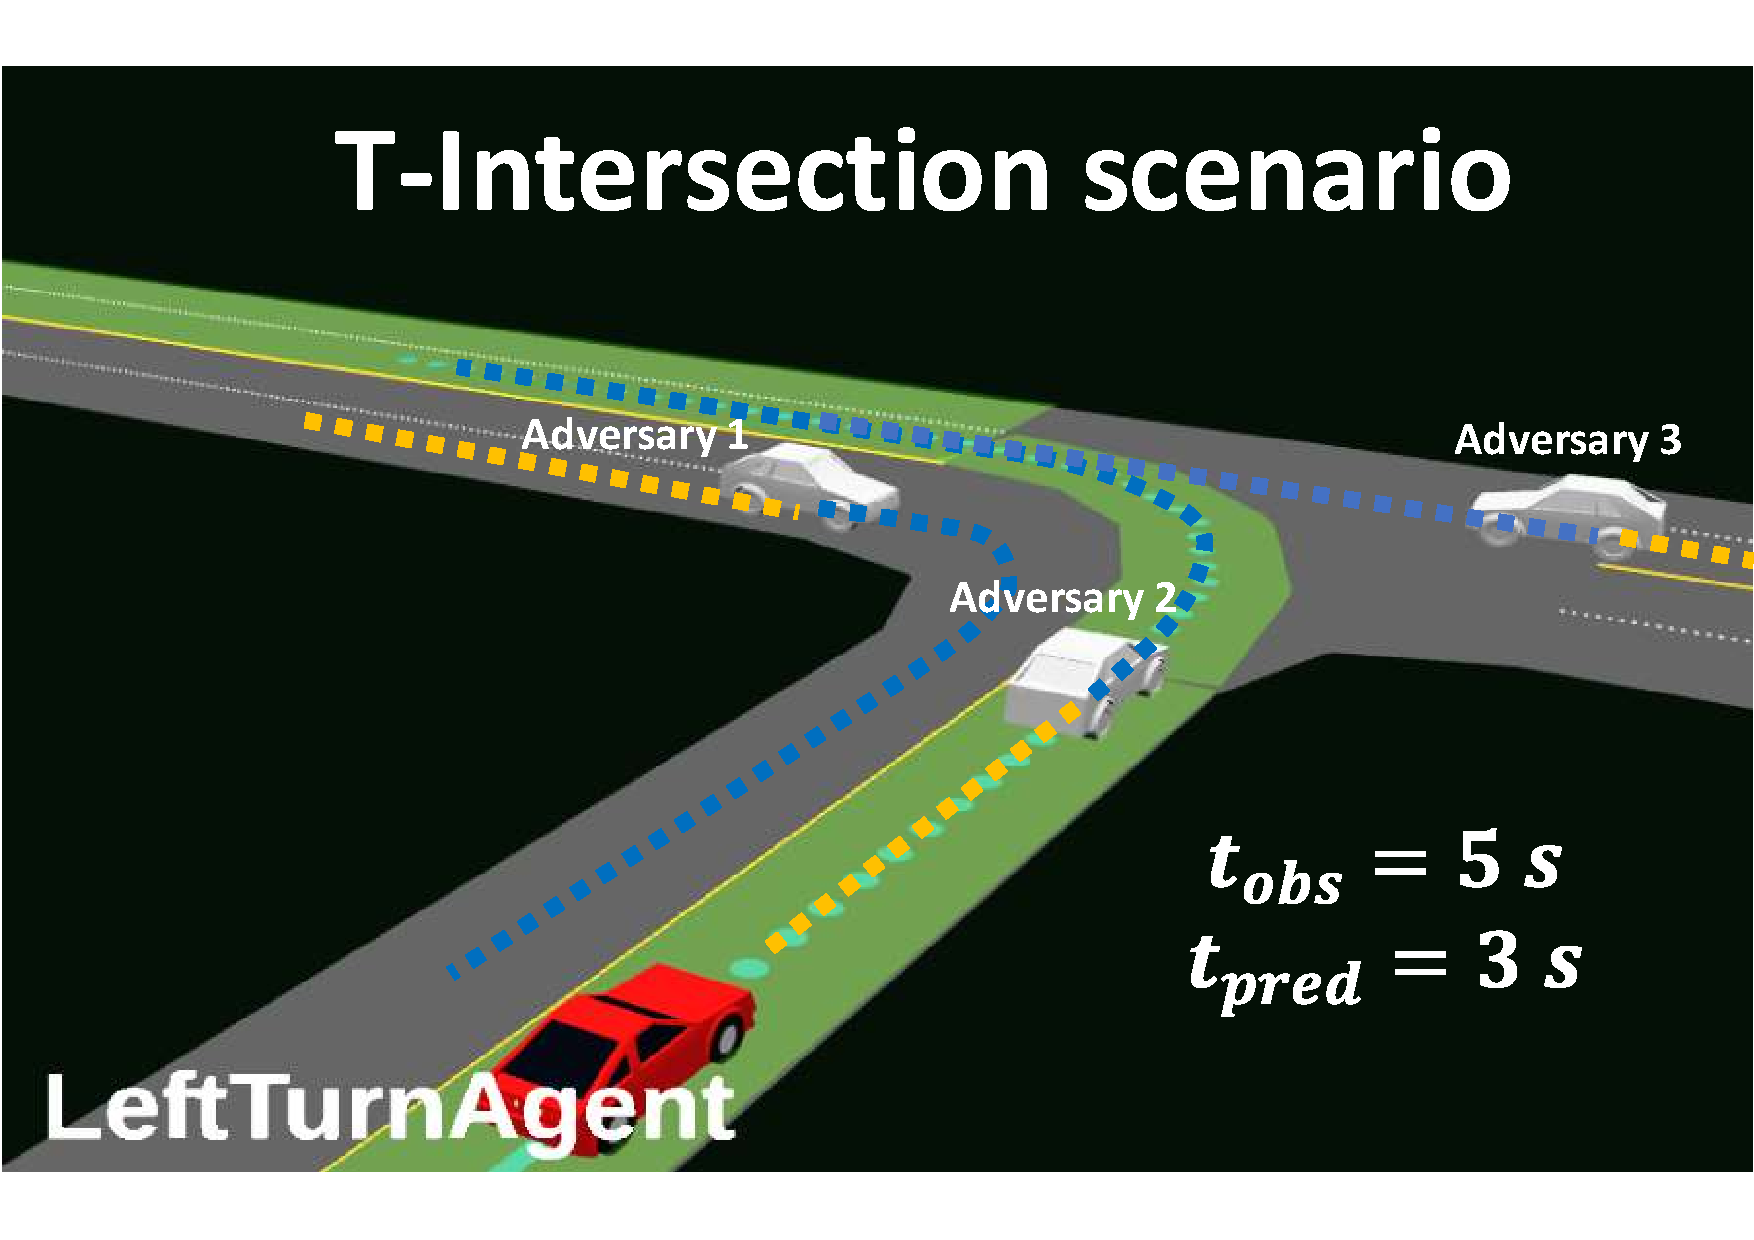
\includegraphics[width=0.45\textwidth]{chapter_8_Applications/dm_t-intersection_scenario.pdf}
	\caption{Simulation environment. A visualization of the ego-vehicle driving in the T-intersection scenario. The past positions of the adversaries (\textbf{\color{YellowOrange}{yellow}}) and the predicted trajectories (\textbf{\textcolor{blue}{blue}}) are represented in the scenario.}
	\label{fig:chapter_8_Applications/dm_t-intersection_scenario}
\end{figure}

In recent years, RL has emerged as a promising approach for developing decision-making policies for AVs \cite{Mnih2015}, outperforming ruled-based approaches that usually cannot solve complex situations \cite{Zhu2019}. However, a large number of interactions with the environment are required to obtain the desired policy. This is why other approaches such as imitation learning \cite{SilverHuangEtAl16nature} and inverse RL \cite{Ross2010}, based on human experts' behaviours are also used in the literature. 

This work is focused on a critical issue for RL-based AVs, which is the state representation problem. Traditional state representations often focus on low-dimensional features such as distance to obstacles, lane positions, and vehicle velocities \cite{Rodrigo2023}. However, these representations may not be sufficient to capture the complex interactions among different agents and road structures in urban driving scenarios. To address the state representation problem, some methods have been proposed that use higher-dimensional or learned representations, such as convolutional neural networks \cite{Johan2018} and recurrent neural networks \cite{Tram2018}; other methods have been proposed to use more detailed representations, such as  Bird-Eye-View images \cite{zhang2021endtoend}, image augmentation \cite{kostrikov2021image} or occupancy grids \cite{moghadam2019hierarchical}. These methods have shown promising results in improving the generalization and robustness of the decision-making approaches. Recently, transformer-based approaches have gained increasing attention for their ability to capture long-term dependencies and interactions among different entities in sequential data. In the context of AVs, transformers have been used to reduce the computational load in end-to-end approaches \cite{Li4} and anticipate future states with prediction-aware planning \cite{valiente2022predictionaware}.

\begin{figure}[h]
	\centering        
	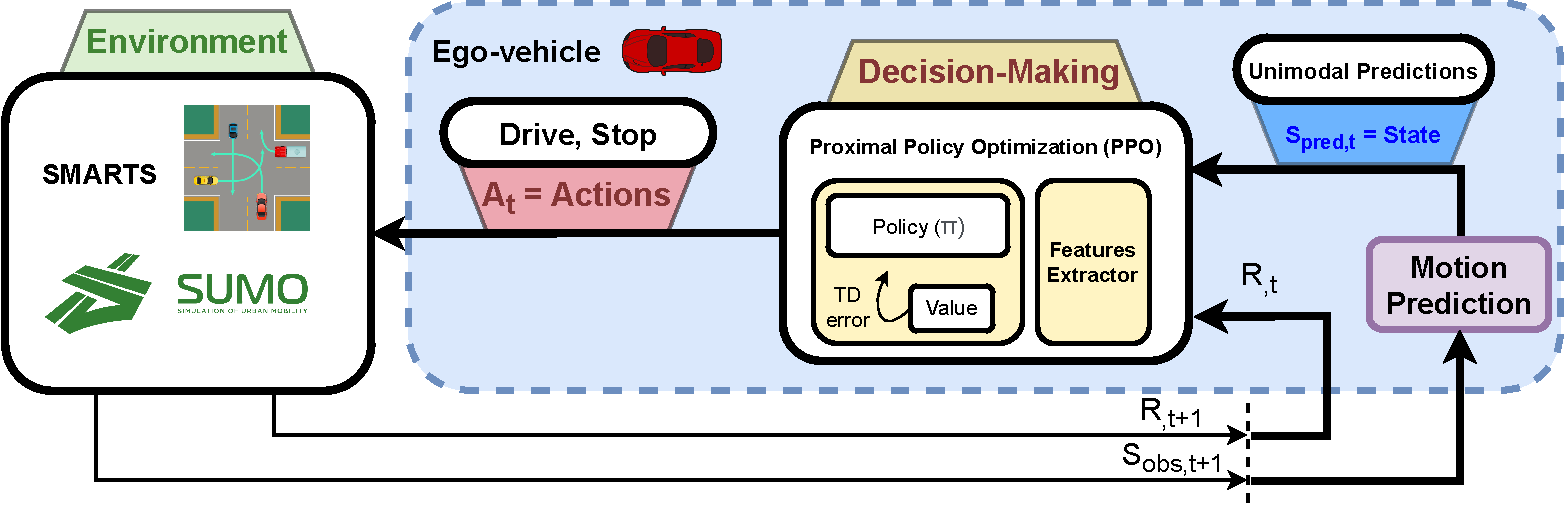
\includegraphics[width=0.95\textwidth]{chapter_8_Applications/dm_prediction_framework.pdf}
	\caption{An overview of the Augmented Reinforcement Learning with Efficient Social-based Motion Prediction for Autonomous Decision-Making. The observations (both position and ID, so, trackers) of the vehicles in the scenario are obtained from the simulator. The MP module estimates the future positions of these vehicles, taking into account the most plausible score of a multimodal prediction. The decision-making module selects high-level actions based on this information. These actions are executed by the simulator, which provides a new state to the framework. }
	\label{fig:chapter_8_Applications/dm_prediction_framework}
\end{figure}

The objective of this study is to illustrate the efficacy of employing a low-dimensional state representation in conjunction with an MP method. We aim to prove that the proposed framework can lead to good performance in urban scenarios. More specifically, we present the following contributions:

\begin{itemize}
	\item The augmentation of RL techniques with MP to improve state representation. By predicting vehicle trajectories, we can better capture the complex interactions between different agents and road structures in urban driving scenarios. 
	
	\item Higher explainability than end-to-end methods. Intermediate states are accessible in our approach. This can help to understand the decisions made.
	
	\item We provide a comparison with baseline methods in a standard scenario. We demonstrate that our approach leads to some improvements in performance, particularly in scenarios with high velocities.
\end{itemize}
	
The RL framework proposed in this work, which executes high-level decisions to solve urban driving scenarios, is represented in Fig. \ref{fig:chapter_8_Applications/dm_prediction_framework}. The past observations of the position of adversaries are obtained from the environment. This information is provided to the MP module, which estimates future positions. The PPO algorithm takes these predictions and generates the decision-making output.

We propose two different learning processes: supervised learning for the motion prediction module and a reinforcement learning approach for the decision-making module. These two modules are trained separately, which allows access to the information of the predictions that feed the decision-making module.

\begin{figure}[h]
	\centering
	\setlength{\tabcolsep}{2.0pt}
	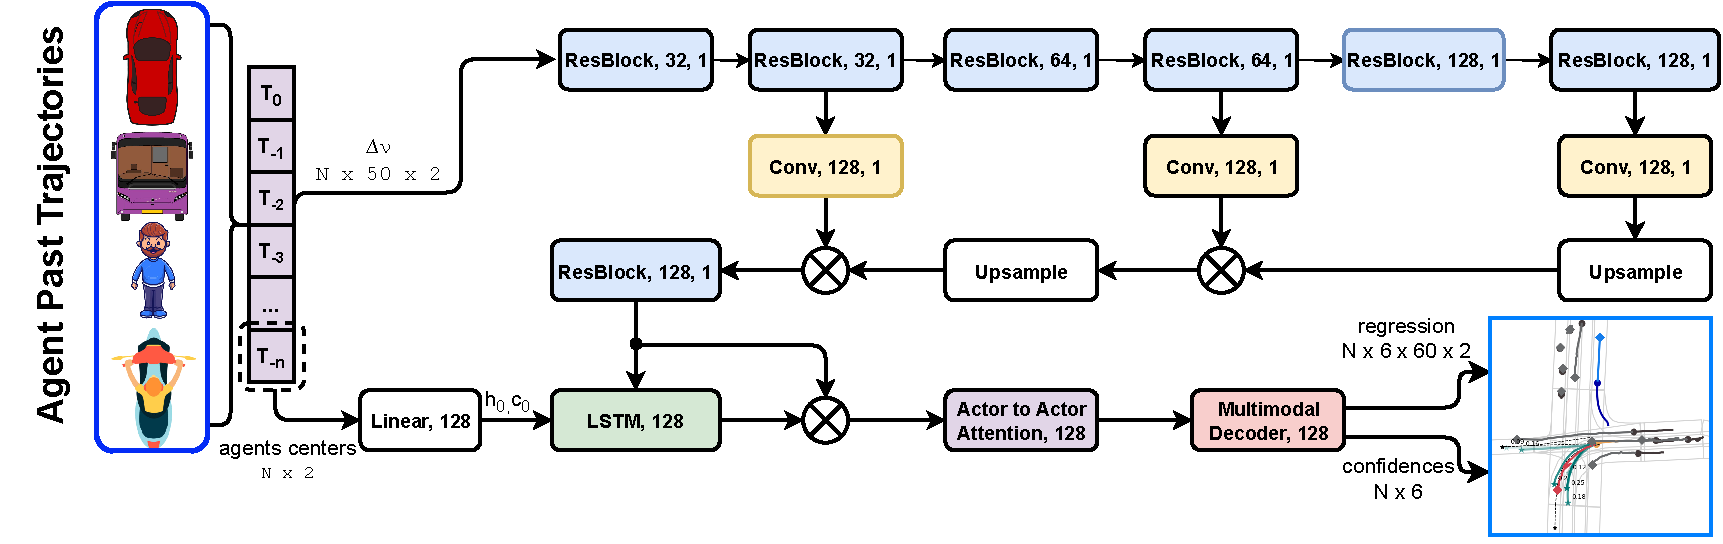
\includegraphics[width=\linewidth]{chapter_8_Applications/social_prediction_baseline.pdf}
	\caption{Overview of our Efficient Social-based Motion Prediction. The main inputs are the relative displacements and centers (last observations) of the agents in the ego-vehicle frame. The relative displacements and centers are encoded through a sequence of Residual, Convolutional Blocks, LSTM and Attention module. Finally, a multimodal decoder based on residual blocks is used to predict \textit{K} final future trajectories (modes) and their confidence scores.}
	
	% On the other hand, the agents centers are encoded through a linear layer to initialize the hidden and cell vector of the LSTM layer, which processes the previously latent motion history
	\label{fig:chapter_8_Applications/social_prediction_baseline}
\end{figure}

Predicting the future behaviour of traffic agents \cite{wilson2023argoverse} around the ego-vehicle is one of the key unsolved challenges in reaching full self-driving autonomy. In that sense, an Autonomous Driving Stack (ADS) can be hierarchically broken down into the following tasks: (i) perception, responsible for identifying what is around the vehicle, then track and predict what will happen next, (ii) planning and decision-making, deciding what the AD stack is going to do in the near future and (iii) control, that sends the corresponding low-level commands (brake, throttle and steering angle) to the vehicle. 

This prediction is required to be multi-modal, which means given the past motion of a particular vehicle and its surrounding scene, there may exist more than one possible future behaviour (also known as modes). Therefore, MP models need to cover the different choices a driver could make (i.e. going straight or turning, accelerations or slowing down) as a possible trajectory in the immediate future or as a probability distribution of the agent's future location. In other words, when an ADS attempts to make a specific action (e.g. left turn), it must consider the future motion of the other vehicles, since the own future actions (also known as decision-making or behaviour planning) depends on the all possible maneuvers of the other agents of the scene for safe driving. %In our case, though we train the MP model in a multi-modal way, we provide the best mode (trajectory with the highest confidence).

Since our proposed pipeline (Fig. \ref{fig:chapter_8_Applications/dm_prediction_framework}) is multi-stage to provide a more interpretable framework, we follow the principles of the Argoverse 2 Motion Forecasting dataset \cite{wilson2023argoverse} to train our prediction model. In our case, we build an efficient model solely based on past trajectories (motion history, $obs_{len} = 50$) and agents interactions, taking into account the corresponding traffic rules, not requiring fully-annotated HD map information, to predict $obs_{len} = 60$ future steps. % Given the standard frequency of 10 Hz, this makes 5s and 6s of observation and prediction respectively. 

The SMARTS \cite{SMARTS} framework provides only the positions of the agents in the timestamp \textit{t}. Nevertheless, in order to predict the future $pred_{len}$ trajectories of the agents, we require their corresponding $obs_{len}$ trackers over a certain set of observations. Most vehicle prediction datasets \cite{wilson2023argoverse} aim to predict the future behaviour of a target agent assuming the surrounding agents have been detected and tracked (so, monitored over time) and the map information is also provided. In that sense, since SMARTS provide the agents in the same order for consecutive timestamps (that is, the agent 5, unless it disappears from the scene, will be the agent 5 again in the next frame), we are able to compute a FIFO (\textit{First Input First Output}) for each agent, not requiring data association \cite{kuhn1955hungarian} to perform this task. 

On top of that, as proposed by multiple methods \cite{liang2020learning, gomez2023improving}, we consider only the vehicles that are observable at \textit{t=0}, handling those agents that are not observed over the full sequence spectrum (observation length = \textit{$obs_{len}$} + prediction length = \textit{$pred_{len}$}) by concatenating a binary flag $b_i^t$ that indicates if the agent is padded or not. In particular, we filter the static elements and track fragments scored by Argoverse 2 to get only the most relevant traffic agents, reducing the number of agents to be considered in complex traffic scenarios. Furthermore, to make the model translation and rotation invariant, the coordinate system in our model is BEV-centered of a given target agent at $t = 0$, and we use the orientation from the target location given in the same timestamp as the positive $x$-axis. Note that this representation will benefit the model to have a common representation to enhance the generalization of the model and prevent overfitting. Once the scene has been translated and rotated, instead of using absolute 2D-BEV (\textit{xy} plane), the input for the agent \textit{i} is a series of relative displacements:

\begin{equation}
	\Delta \boldsymbol{\nu}^{t}_i = \boldsymbol{\nu}^{t}_i - \boldsymbol{\nu}^{t-1}_i
\end{equation}

Where $\boldsymbol{\nu}^{t}_i$ represents the state vector (in this case, \textit{xy} position of the agent \textit{i} at timestamp \textit{t}).

Since our model focus on an efficient encoding of the social information, we base our model on the ActorNet backbone proposed by \cite{liang2020learning}, as observed in Fig. \ref{fig:chapter_8_Applications/social_prediction_baseline}. While both CNNs and RNNs can be used for temporal data, ActorNet uses an 1D CNN to process the trajectory input for its effectiveness in extracting multi-scale features and efficiency in parallel computing. The output is a temporal feature map, whose element at $t=0$ is used as the actor feature. The network has $3$ groups/scales of 1D convolutions. Each group consists of $2$ residual blocks, with the stride of the first block as $2$. Then, a Feature Pyramid Network (FPN) \cite{lin2017feature} is used to fuse the multi-scale features, and apply another residual block to obtain the output tensor. For all layers, the convolution kernel size is $3$ and the number of output channels is $128$. Layer normalization and the Rectified Linear Unit (ReLU) are used after each convolution. 

On top of that, in a similar way to \cite{wang2022ganet}, the agents centers (observations at $t=0$) are encoded through a linear layer to initialize the hidden and cell vector of the LSTM layer, which processes the previously latent motion history. After that, a social attention block is used to compute the most representative agents interaction.

Taking the final actor features after motion history and agents interaction, a multi-modal prediction header outputs the final motion forecasting. For each agent, it predicts $K$ possible future trajectories and their confidence scores. The header has two branches, a regression branch to predict the trajectory of each mode and a classification branch to predict the confidence score of each mode.

For the $m$-th actor, a residual block and a linear layer in the regression branch to regress the $K$ sequences of BEV coordinates is obtained:

\begin{equation}
	O_{m, \text{reg}} = \{ (\mathbf{p}_{m,1}^k, \mathbf{p}_{m,2}^k, ..., \mathbf{p}_{m,T}^k) \}_{k \in [0, K-1]}
\end{equation}

where $O_{m, \text{reg}}$ is the whole set of regressions and $\mathbf{p}_{m,i}^k$ is the predicted $m$-th actor's BEV coordinates of the $k$-th mode at the $i$-th time step.

On the other hand, for the classification branch, a MLP to $\mathbf{p}_{m,T}^k - \mathbf{p}_{m,0}$ to get $K$ distance embeddings is applied. Finally, each distance embedding is concatenated with the actor feature, applying a residual block and a linear layer to output $K$ confidence scores, $O_{m, \text{cls}} = (c_{m,0}, c_{m,1}, ..., c_{m,K-1})$.

In this particular work, we take the most plausible future trajectory for each agent (both the adversaries and the ego-vehicle) in the following timestamps: \textit{t=0}, \textit{t=10}, \textit{t=20} and \textit{t=30}, which correspond to the current position and the predicted position of the corresponding agent 1, 2 and 3 seconds in the future respectively. Even though we train our prediction model following the principles of Argoverse 2 (5s and 6s of observation and prediction respectively), given the velocities and traffic density of the experiments run in the SMARTS simulator , we believe that predicting 3s in the future is enough for this purpose to evaluate the high-level actions of decision-making layer preventing overfitting. In future works, we will design more difficult scenearios, up-to-pair with the Argoverse 2 dataset (specially in terms of intersections or lane change behaviours at high speed) where multimodal predictions with higher prediction horizons will be required.

A Markov Decision Process (MDP) is a discrete-time stochastic control process that provides a mathematical framework for modelling decision-making environments. An MDP is a tuple $(S,A,P,R)$ in which $S$ is a set of states named state space, $A$ is a set of actions named action space, $P$ is the probability function and $R$ is a reward function. An algorithm with a given state $s \in S$ takes an action $a \in A$ transitioning to $s'$ with a probability $P(s,a,s')$, and getting a reward $R(s,a,s')$ as shown in Fig. \ref{fig:chapter_8_Applications/dm_prediction_framework}. This algorithm iterates through this loop to learn a desired behaviour. 

The goal in an MDP is to find a good policy for the decision-making system. The objective is to find the optimal policy $\pi*(s)$, that maximizes the cumulative function of the future reward.

We represent the driving scenario as an MDP to develop our decision-making module. We consider the output of the MP module as an input to this module. The state space, action space, and reward functions are defined in this section.

The state is defined by the predicted trajectories of the ego-vehicle and the five closest vehicles in the scenario.
\begin{equation}
	s_t = (K^{ego}_t, K^1_t, ..., K^{5}_t)
	\label{eq:state}
\end{equation}

where $K^{i}_t = (x^i_{t_0}, y^i_{t_0}, x^i_{t_1}, y^i_{t_1}, x^i_{t_2}, y^i_{t_2}, x^i_{t_3}, y^i_{t_3})$ contains the future estimations of the positions of the vehicles across a future horizon of three seconds. A representation of a state vector is shown in Fig \ref{fig:chapter_8_Applications/dm_state}, where the vehicles' predicted positions are represented.

\begin{figure}[h]
	\centering
	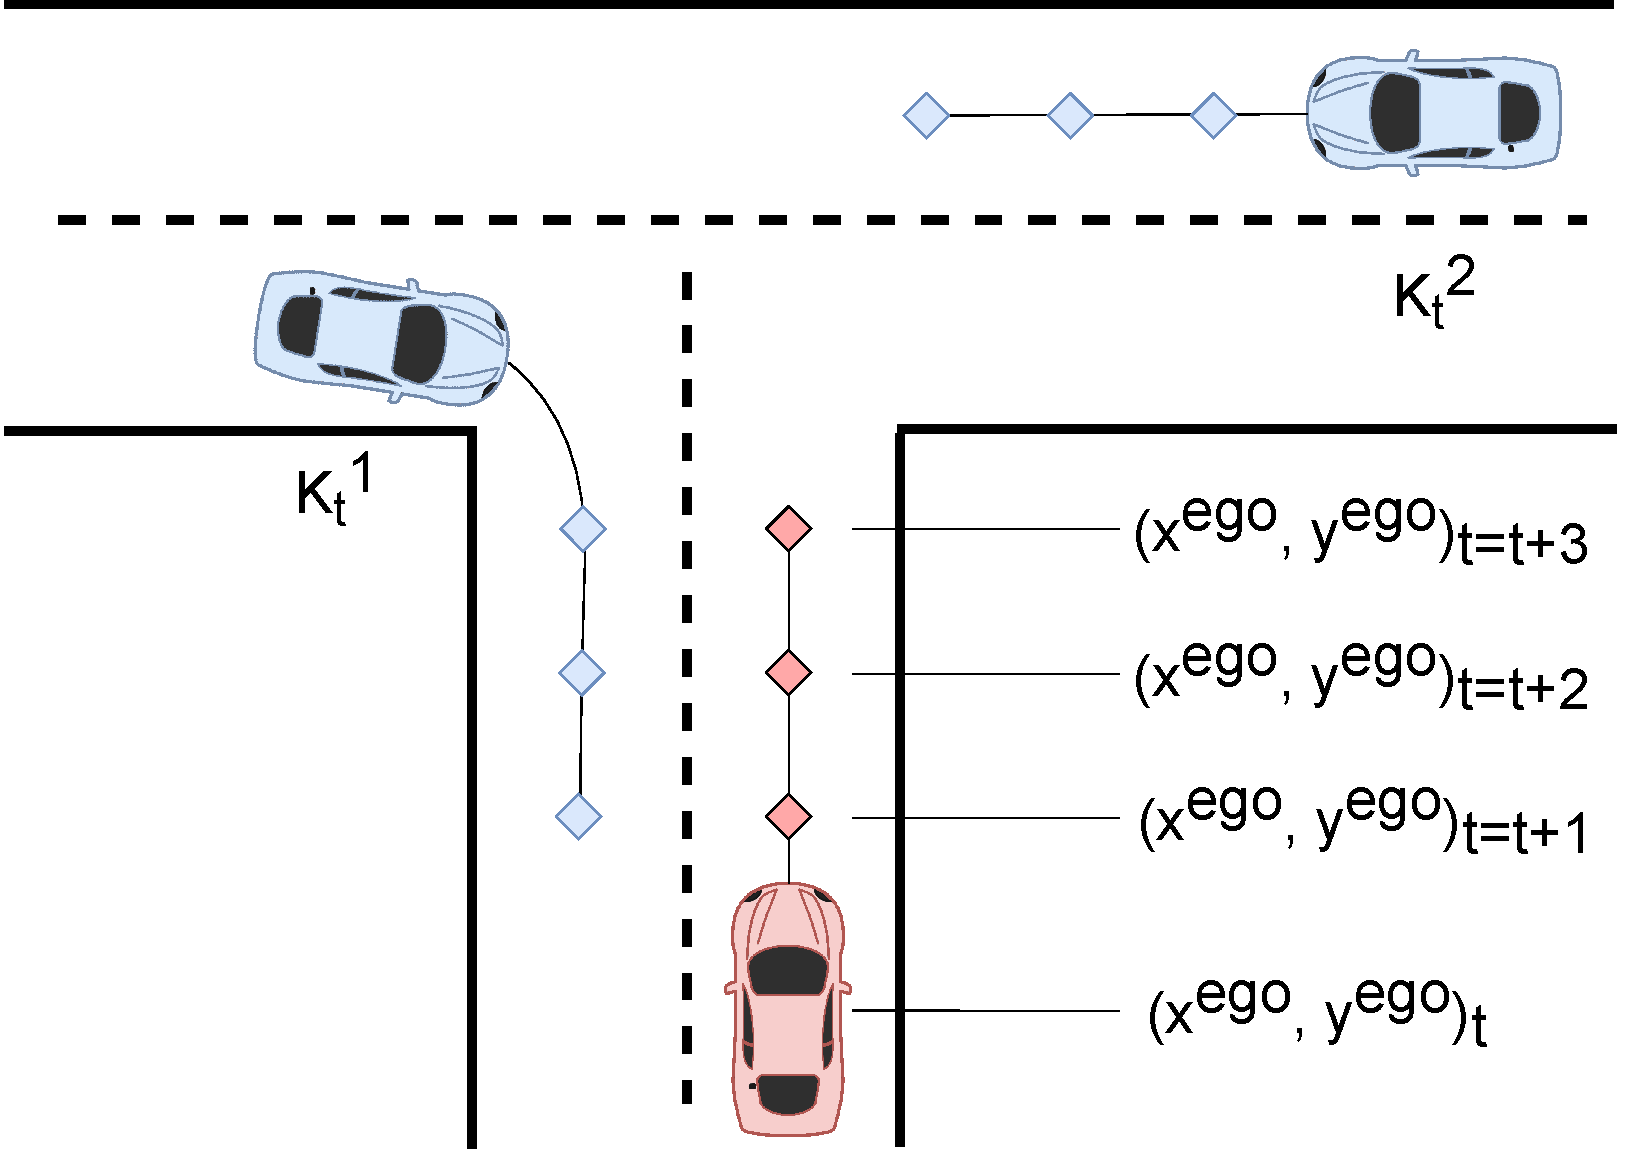
\includegraphics[width=0.40\textwidth]{chapter_8_Applications/dm_state.pdf}
	\caption{The ego-vehicle (\color{brickred}{red}) and the adversaries (\color{cadetblue}{blue}) predicted positions in the next three seconds are represented.}	
	\label{fig:chapter_8_Applications/dm_state}
\end{figure}

We propose a discrete action space formed by two actions. A low-level controller implemented by the simulator is in charge of performing smooth driving based on these actions. These actions are focused on the ego-vehicle velocity. The first action aims to reach a desired predefined velocity and the second action reduces the velocity until the vehicle stops. The action space is defined as:

\begin{equation}
	a=(Drive, Stop)    
	\label{eq:action}
\end{equation}

\subsubsection{Reward Function}
The reward function is defined in terms of success or failure. A negative reward is given when there is a collision and a positive reward is given when the vehicle reaches the success point, situated at the end of the scenario.

\begin{equation}
	r = k_v * v_{ego} + \left\lbrace\begin{array}{lcc}
		1 & if & sucess \\ 
		-1 & if & collision \\
	\end{array}\right.
	\label{eq:Reward}
\end{equation}

As shown in Equation \ref{eq:Reward}, we add one more factor to the reward function to encourage the ego-vehicle to move. We propose a cumulative reward based on its longitudinal velocity. We use a constant small enough to ensure that the reward per episode is bounded between -1 and 1.

Our approach for the RL implementation (Fig. \ref{fig:chapter_8_Applications/dm_RL_network}) builds upon our previous research \cite{Gutierrez2022}, where we demonstrated that incorporating a feature extractor module to a PPO algorithm yields improved metrics and faster convergence. 

\begin{figure}[h]
	\centering
	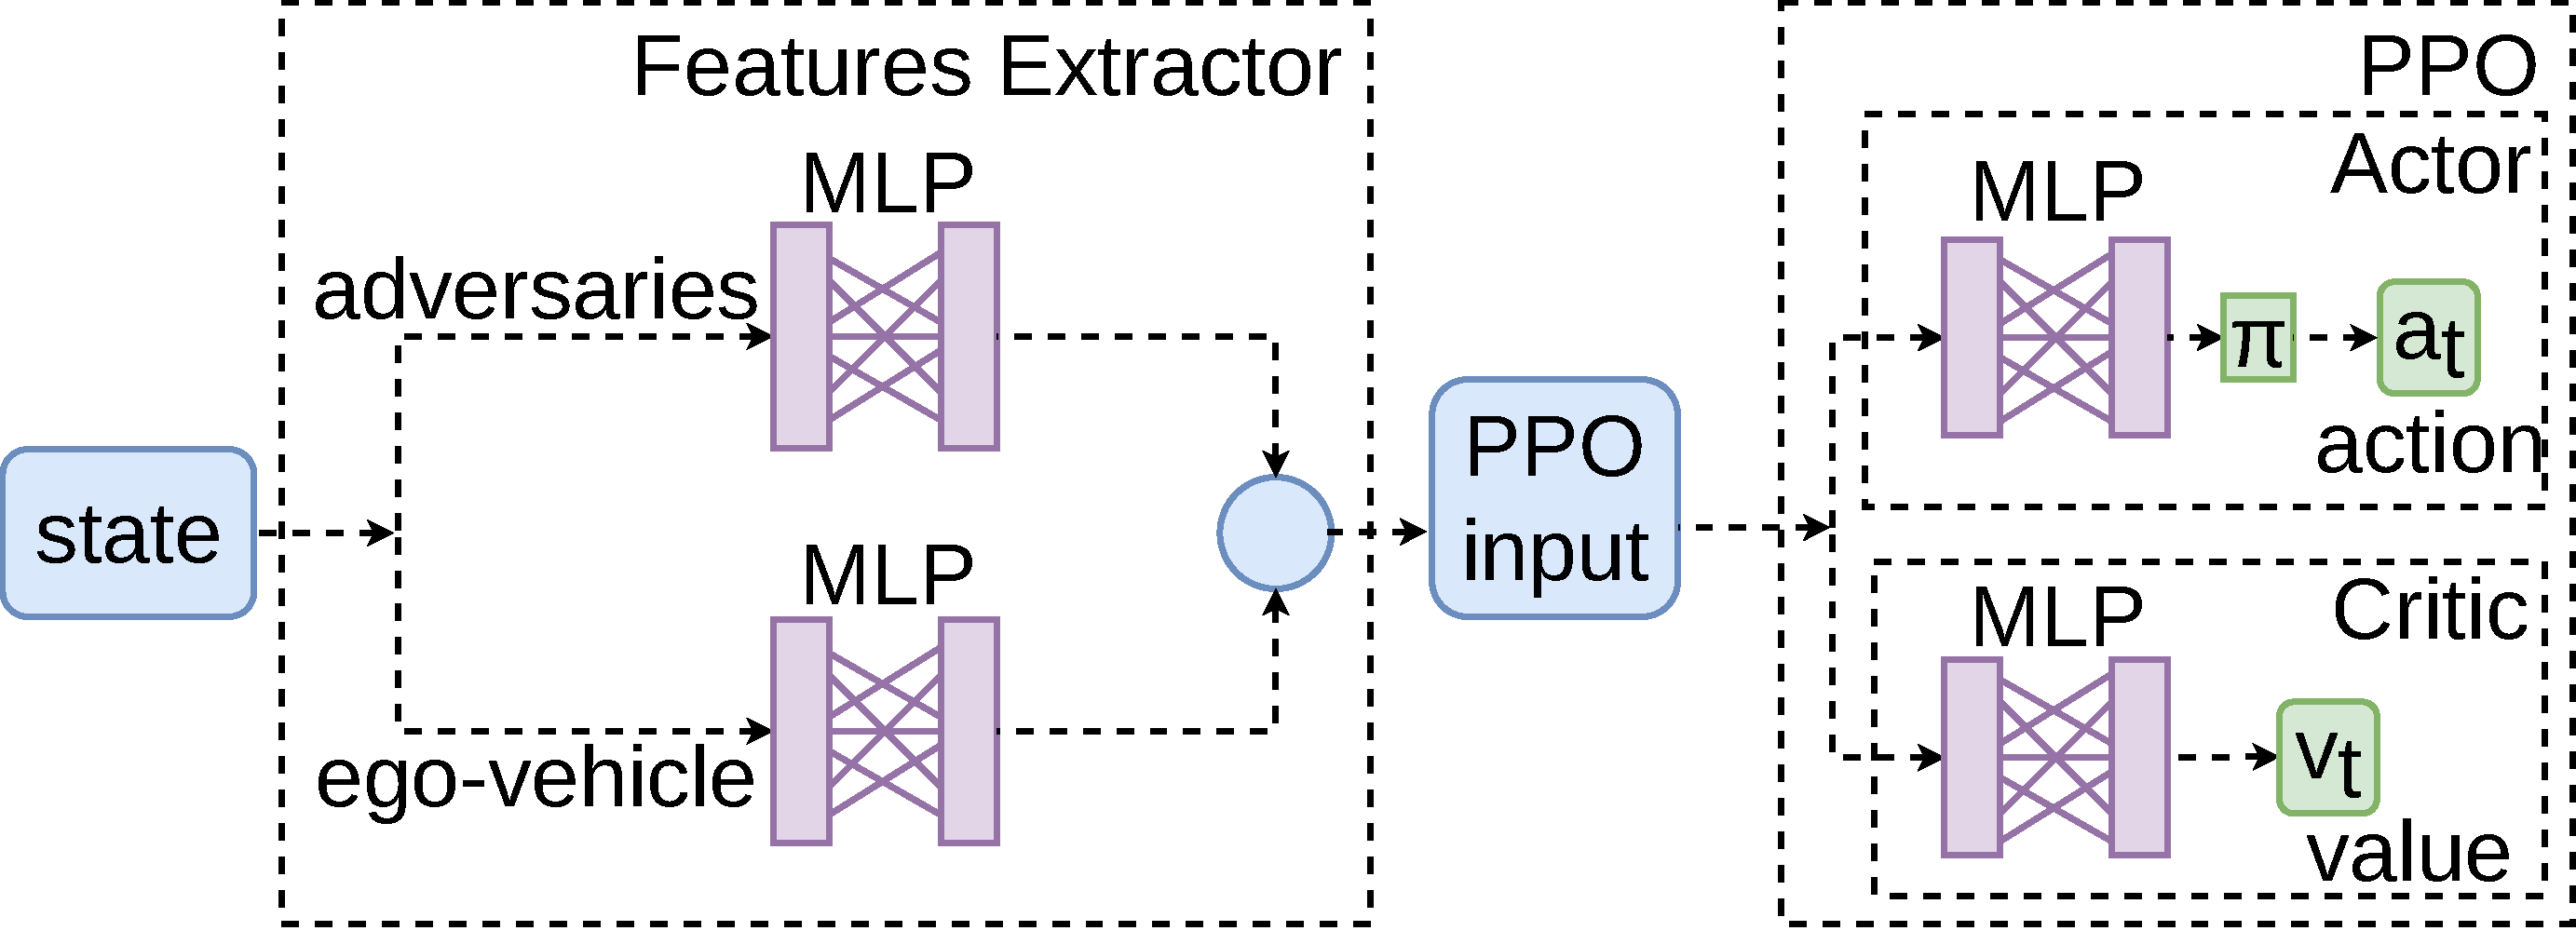
\includegraphics[width=0.45\textwidth]{chapter_8_Applications/dm_RL_network.pdf}
	\caption{The neural network architecture consists of two fully connected layers followed by the concatenation of both adversaries and ego vehicle features. The resulting concatenated features are then passed through an actor-critic structure, which comprises two layers, each containing 128 neurons.}	
	\label{fig:chapter_8_Applications/dm_RL_network}
\end{figure}

In this implementation, we introduce separate feature extractors for adversaries and the ego-vehicle, which are then concatenated into the input for the PPO algorithm. This algorithm consists of two models: the Actor, responsible for selecting an action based on the policy, and the Critic, which estimates the value function.

To validate the performance of our approach, an intersection scenario is implemented in SMARTS, which is a SUMO \cite{Sumo} based simulation platform for research on autonomous driving.

\begin{figure}[h]
	\centering        
	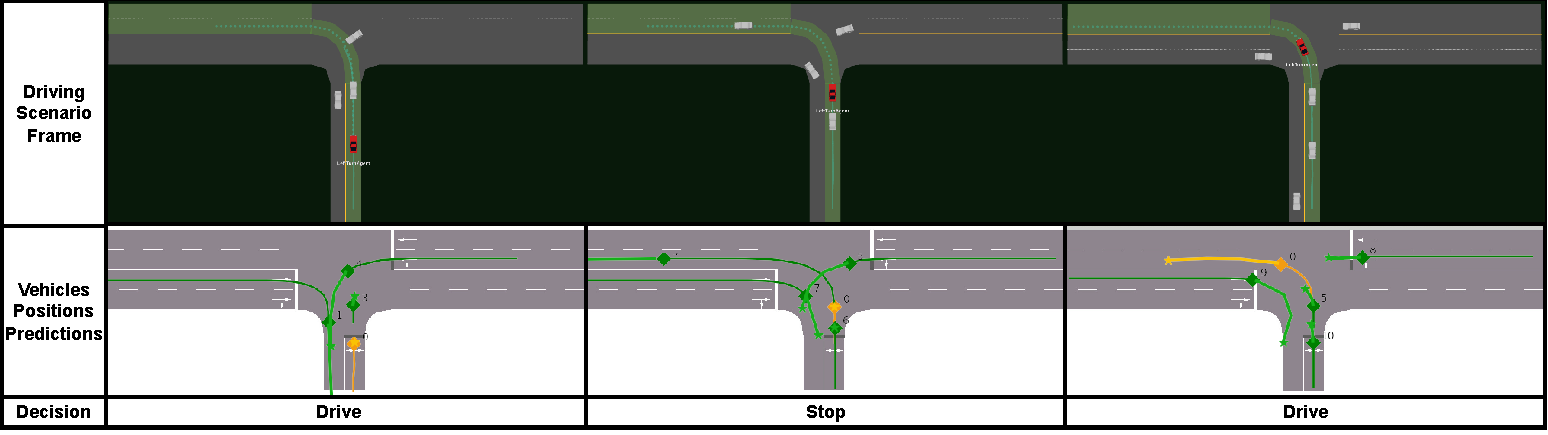
\includegraphics[width=0.95\textwidth]{chapter_8_Applications/dm_prediction_results.pdf}
	\caption{Simulation overview of our system behaviour. The red car follows the green path, and each image represents a different frame of the simulation. We also show the predicted positions below each image and the actions taken by the decision-making module.}
	\label{fig:chapter_8_Applications/dm_prediction_results}
\end{figure}

The scenario is an urban unsignalized T-intersection. The objective is to execute a left turn maneuver in the absence of traffic signal protection, allowing the continuous flow of traffic. Fig. \ref{fig:chapter_8_Applications/dm_t-intersection_scenario} illustrates the drivable area (highlighted in green) where the ego-vehicle can navigate to reach the target location. Simulations are reset under three conditions: 1) the ego-vehicle successfully reaches the target, 2) the episodic step surpasses the maximum time steps limit, and 3) the ego-vehicle collides or deviates from the drivable route.

We define different scenario configurations to test the performance of the proposed framework. First, the regular T-intersection scenario which is defined in SMARTS, where a random number of vehicles between [5-10] are spawned every minute, and the maximum velocity of these vehicles is 14 km/h. Then, we propose different configurations increasing the maximum velocity of the adversaries to 30, 60, and 90 km/h. 

In decision-making, the success rate serves as a direct measure of the effectiveness of the RL agent in accomplishing the designated task. Besides, the average time of the episode is a common metric used in the literature. These metrics are defined as:

\begin{itemize}
	\item $success~[\%] = n_{success}/n_{success}$
	\item $t_{e} [s] = \sum{t_{n}}/n_{episodes}$
\end{itemize}

where the number of episodes $n_{e}$ is 100 and simulation time is measured in seconds. 

To evaluate the performance of our approach we first present a comparison with the existing methods for decision-making in the literature and then an ablation study is conducted. 

This first study compares the proposed approach with other existing methods for decision-making. The baseline methods used for comparison are Data-regularized Q-learning (DrQ) \cite{kostrikov2021image}, Soft Actor-Critic (SAC) \cite{haarnoja2019soft}, and PPO. These methods have different features and serve as reference points for evaluating the proposed approach. The results presented in Table \ref{table:comp} demonstrate a higher success rate of our proposal.

\begin{table}[h!]
	\centering
	\caption{A comparison of the proposed framework against the existing baselines in the T-intersection scenario. The success rate S[\%] and the average episode time $t_{e}$ are presented.}
	\label{table:comp}
	\setlength{\extrarowheight}{2pt}
	\begin{tabular}{cccccc} 
		\ChangeRT{1pt}
		Metric & Ours & PPO & SAC & DrQ\\
		\hline 
		S[\%] & \textbf{80} & 70 & 68 & 78 \\ 
		$t_{e}$(s) & 22.3 & 36.4 & 19.2 & 18.2 \\
		\hline
		\ChangeRT{1pt}
	\end{tabular}
\end{table}

Two ablative studies are carried out to see how the use of motion prediction in the state representation can improve the performance of the framework. The first approach is to use just the position of the vehicles as the input to the decision-making module and the second approach is to use the locations over the past five seconds. We test the three approaches under the previously introduced configurations with different adversaries' velocities, from 15km/h to 90km/h. To correctly evaluate the performance of the decision-making system we propose different metrics that aim to provide a better comprehension of the behaviour. We believe that the success rate is still a good indicator, but we slightly modify the average time, only considering the successful episodes to calculate this metric. In addition, we include a new relevant metric: the average ego-vehicle velocity when a collision takes place $v_{c}$.  

The results presented in Table \ref{table:chapter_8_Applications/dm_ablation_study_smarts} show that the use of the predicted positions in the state vector avoids more collisions as the velocities increase. Besides, the average collision velocity and the average time to complete the scenario are lower for the proposed approach. 

\begin{table}[h]
	\centering
	\caption{An ablation study comparing three state representations with the different scenario configurations: Current positions, Past positions, and Future positions. The success rate S[\%], the episode time $t_{e}$ in these successful episodes, and the average velocity of collision $v_{c}$ are presented.}
	\label{table:8_dm_ablation_study_smarts}
	\setlength{\extrarowheight}{2pt}
	\begin{tabular}{cccccc} 
		\ChangeRT{1pt}
		& Metric & 15 km/h & 30 km/h & 60 km/h & 90 km/h  \\
		\hline 
		\multirow{3}{*}{Future}
		&S [\%] & 80 & 78 & 78 & 77 \\ 
		&$t_{e}$ (s) & 22.3 & 23.3 & 23.4 & 23.3 \\
		&$v_{c}$ (km/h) & 4.9 & 5.1 & 5.6 & 5.6 \\
		\hline
		\multirow{3}{*}{Current}
		&S [\%] & 77 & 73 & 70 & 70 \\ 
		&$t_{e}$ (s) & 25.1 & 23.4 & 23.4 & 23.3 \\
		&$v_{c}$ (km/h) & 5.1 & 5.5 & 6.1 & 6.2 \\
		\hline
		\multirow{3}{*}{Past}
		&S [\%] & 78 & 75 & 72 & 71 \\ 
		&$t_{e}$ (s) & 24.2 & 23.3 & 23.2 & 23.1 \\
		&$v_{c}$ (km/h) & 4.9 & 5.2 & 5.9 & 6.0 \\
		\hline
		\ChangeRT{1pt}
	\end{tabular}
\end{table}

Finally, an overview of the behaviour of our system is shown in Fig. \ref{fig:chapter_8_Applications/dm_prediction_results}. The ego-vehicle in red follows the trajectory defined in green. Each image represents a different frame of the simulation and the respective predictions of the positions are displayed below. Besides, the action executed by the decision-making module for each frame is shown.

The proposed method incorporates an Efficient Social-based Motion Prediction module, which predicts the future positions of vehicles within the scenario. These predictions improve a Reinforcement Learning-based Decision Making module. The results of the study demonstrate that our approach achieves significant performance improvements, particularly in scenarios involving high velocities.

This research opens up several potential directions for future work. The proposed approach can be evaluated in a broader range of urban driving scenarios to assess its robustness and scalability, up-to-pair with the difficulty of the Argoverse 2 dataset scenarios (specially in terms of intersections or lane change behaviours at high speed) where multimodal predictions with higher prediction horizons will be required. Furthermore, the Reinforcement Learning-based Decision Making module can be enhanced by exploring advanced algorithms.

\section{Holistic Simulation in CARLA}
\label{sec:8_holistic_simulation}

The main contribution of our AD PerDevKit is the creation of a ground-truth generation tool for the surrounding obstacles of the ego-vehicle using CARLA and ROS. For its implementation, as explained in section \ref{dosovitskiy2017carla}, the CARLA-ROS brige is used so that the simultaneous execution of CARLA and this tool is not necessary, since the execution of both programs can be very demanding due to the simulator requirements. This way it is possible to record a rosbag (a file with all the ROS messages) with the GT information, so that only an area around the ego-vehicle is analyzed and not the whole obstacles in the CARLA runtime.

The messages created by CARLA contain the information of the different objects of the environment in relation to the map on which it is being used. However, to be used independently, the obstacles must be referenced to the ego-vehicle. Therefore, it is necessary to perform the different transformations to go from a coordinate system based on the map to a coordinate system based on the ego-vehicle.

\subsection{Method for obtaining 2D bounding boxes}
While the CARLA-ROS bridge gives access to the 3D bounding boxes of the objects in the environment, it does not provide the projected 2D bounding boxes of these 3D objects in the camera. We perform a series of transformations to go from the coordinates of the world to the pixels containing that object within each image generated by the camera.

\begin{figure}[h]
	\centering
	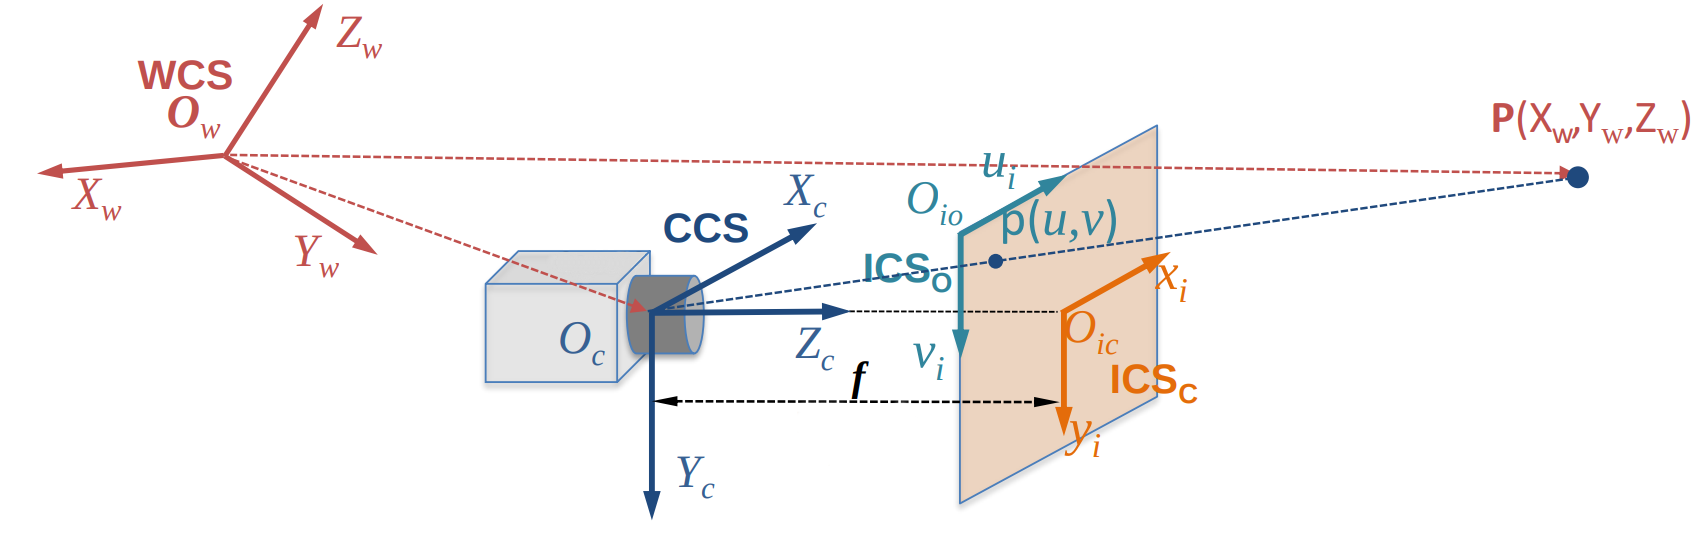
\includegraphics[width=0.48\textwidth]{chapter_8_Applications/ad_perdevkit_change_of_coordinates_from_world_to_camera.png}
	\caption{Geometry transformation from world to camera}
	\label{fig:chapter_8_Applications/ad_perdevkit_change_of_coordinates_from_world_to_camera}
\end{figure}

A conversion from the world coordinates to the image ones is necessary to transform the eight vertices of a 3D bounding box into the vertices of a 2D bounding box. For this purpose, it is necessary to apply some geometry transformations as shown in Fig. \ref{fig:chapter_8_Applications/ad_perdevkit_change_of_coordinates_from_world_to_camera}.

Using homogeneous coordinates, the correspondence between a 3D point in the World Coordinate System (WCS) and its projected pixel in the Image Coordinate System at origin (ICS$_O$) is calculated applying the following equation:

\begin{center}
	$
	\begin{bmatrix} wu \\ wv \\ w \end{bmatrix}
	=
	M_{3x4}
	\begin{bmatrix} X_w \\ Y_w \\ Z_w \\ 1 \end{bmatrix}
	$
\end{center}
where $M_{(3x4)}=M_{int}M_{ext}$ is the camera projection matrix, formed by the product of intrinsic matrix and extrinsic matrix, defined as follow:
\begin{center}
	$
	M_{int}
	=
	\begin{bmatrix}
		f/dx & 0 & u_0 \\
		0 & f/dy & v_0 \\
		0 & 0 & 1 \\
	\end{bmatrix}
	$
\end{center}
\begin{center}
	$
	M_{ext}
	=
	\begin{bmatrix}
		R_{3x3} & T_{3x1} \\
		0 & 1 \\
	\end{bmatrix}
	$
\end{center}

being $f$ focal distance, $(dx,dy)$ physical size of the pixel, $(u_0, v_0)$ centre of the image in pixels, $T_{3x1}$ translation matrix and $R_{3x3}$ rotation matrix from the world (WCS) to the camera (CCS). 

The steps to perform this conversion are the following:

\begin{enumerate}
    \item Transformation from World Coordinate System to Camera Coordinate System (WCS/CCS):
	
	During the geometric transformation of the world coordinates to the image, homogeneous coordinates are used, such a coordinate system adds a fourth component to the three-dimensional coordinates. This coordinate system has a direct equivalence to the Cartesian coordinate system as shown below.

    \begin{center}
	    $(x, y, z) \rightarrow (x', y', z', w)$\\
        $(x, y, z) = (x'/w, y'/w, z'/w)$
    \end{center}

   Firstly the translation matrix from the world to the camera is obtained.

   \begin{center}
	   $
	   T_{3x1}
	   =
	   \begin{bmatrix} T_x \\ T_y \\ T_z \end{bmatrix}
	   $
	\end{center}

    Afterwards, the rotation matrix is built over the 3 rotation matrices of the different dimensions.

    \begin{center}
	    $ R = R_x(\alpha) R_y(\beta) T_z(\gamma) $
	\end{center}

	Based on the translation matrix and the rotation matrix, a matrix of 4x4 dimensions is built, which together with the matrix of the points to be transformed, gives a matrix with the points in the camera coordinate system.

\begin{center}
	   $
	    P_c
	    =
	    \begin{bmatrix} R_{3x3} & T_{3x1} \\ 0 & 1 \end{bmatrix}
		   \begin{bmatrix} X_w \\ Y_w \\ Z_w \\ 1 \end{bmatrix}
		 =
		   \begin{bmatrix} X_c \\ Y_c \\ Z_c \\ 1 \end{bmatrix}
		  $
\end{center}
	    \item Transformation from Camera Coordinate System to Image Coordinate System in the center of the image (CCS/ICS$_C$):

	    During the transformation to the image coordinate system, it is necessary to work with the distance between the optical center and the image plane, also called focal length. Thereby a matrix is constructed, which together with the points in the camera coordinate system is obtained in the image coordinate system in the center of the image.
	
	    \begin{center}
		    $
		    \begin{bmatrix} wx \\ wy \\ w \end{bmatrix}
		    =
		    \begin{bmatrix}
			    f & 0 & 0 & 0 \\
			    0 & f & 0 & 0 \\
			    0 & 0 & 1 & 0 \\
			    \end{bmatrix}
		    \begin{bmatrix} X_c \\ Y_c \\ Z_c \\ 1 \end{bmatrix}
		    $
		    \end{center}
	    \item Transformation from Image Coordinate System in the center of the image to Image Coordinate System at origin (ICS$_C$/ICS$_O$) in pixels:
	    \par
	    \vspace{1mm}
	    As a last step, the points are transformed to image pixels using the size of the camera sensor as well as the pixel resolution of the image.
	
	    \begin{center}
		    $
		    \begin{bmatrix} wu \\ wv \\ w \end{bmatrix}
		    =
		    \begin{bmatrix}
			    1/dx & 0 & u_0 \\
			    0 & 1/dy & v_0 \\
			    0 & 0 & 1 \\
			    \end{bmatrix}
		    \begin{bmatrix} wx \\ wy \\ w \end{bmatrix}
		    $
		\end{center}
\end{enumerate}
	
After all this, the vertices from the different 3D bounding boxes of the objects in the environment are brought to the pixels of the images taken, and after this, they are transformed to 2D bounding boxes with the vertices furthest from each object.
	
\subsection{Calculation of object visibility}
	One main issue for the GT calculation is that CARLA always render all the objects, even when they are not visible by the camera, LiDAR or Radar, which is a problem for any training process.
	There are many studies about ray tracing that solve this issue. These techniques \cite{raytracing1} \cite{raytracing2} are computationally very expensive so it is very difficult to implement them in real-time.\par
	We propose a method for the calculation of visibility in CARLA and ROS using directly the point cloud calculated by CARLA. A vehicle will be considered as visible, as long as a point of the LiDAR point cloud is found inside an object, in the same way as it is done in the nuScenes dataset \cite{caesar2020nuscenes}. The steps to be performed are the following:
	\begin{enumerate}
		\item Remove objects furthest than the maximum LiDAR distance.
		\item Deletion of the points of the point cloud with the height higher or lower than the objects in the surroundings.
		\item Elimination of points outside the area in which the objects are located, taking into account all possible rotations.
		\item Selection of the visible objects having at least one point in the point cloud taking into account the rotation of the different objects.
	\end{enumerate}
	
	\par
	In order to obtain a much simplified and reduced GT to work with, the tool has been designed with sensor synchronization as the basis. In this way, GT does not have to be calculated every time data is obtained from a sensor, or in certain timestamps in which data is available. Because of this, it is necessary to activate the CARLA synchronization option for the correct functioning of the tool.\par
	
\begin{comment}
	IDEAS:
	
	1. Con el ADS que hay estable, dejarlo otra vez pulido y optimizado en poco tiempo (creo que YOLO está duplicada, PointPillars no corría bien, etc., y eso se puede poner como GT en el R-VIZ, diciendo específicamente que es GT). 
	
	Eso, con el AD-PerDevKit, estimo que fuesen dos días de trabajo.
	
	2. Ya se hicieron pruebas para meter el by-pass de tracking (hecho en SMARTS/SUMO) en CARLA, y funciona bien, aunque hay que retocar.
	
	3. Mi idea es correr el ADS en las rutas del Leaderboard, y obtener scores, sin nada más que lo estable ahora mismo vs meter predicción + dm con RL sobre todo en intersecciones (las decisiones de la red de rodrigo fuera de intersecciones están capadas)
	
	4. Hacer comparativas múltiples:
	
	ADS sin predicción
	ADS sin predicción, con DM en intersecciones (sólo basado en posición)
	ADS con predicción y DM en intersecciones (basado en predicción)
	
	Y la teoría dice que cuanta más capacidad predictiva metas al sistema, mejores deberían ser las métricas holísticas.
	
	Si todo fuese bien, y hasta la fecha de la lectura, mi idea es ayudar al equipo a meter detección, fusión y tracking en simulación y real, aunque no sean integraciones mid-level, y quitar el by-pass, pero lo anterior es más prioritario.
\end{comment}

\section{Summary}
\label{sec:8_summary}